\section{Aukro}

\label{chap:aukro}

Webová aplikace, která se jak napovídá název nezabývá jen aukcemi, ale také normálním prodejem zboží. Protože je to ve své podstatě e-shop, tak od něj očekávám dobře zvolené kategorie, detaily v popise zboží a v případě aukra i výrazné zobrazení hodnocení prodejců zboží.

\subsection{Home page}
\begin{figure}[h]
    \centering
    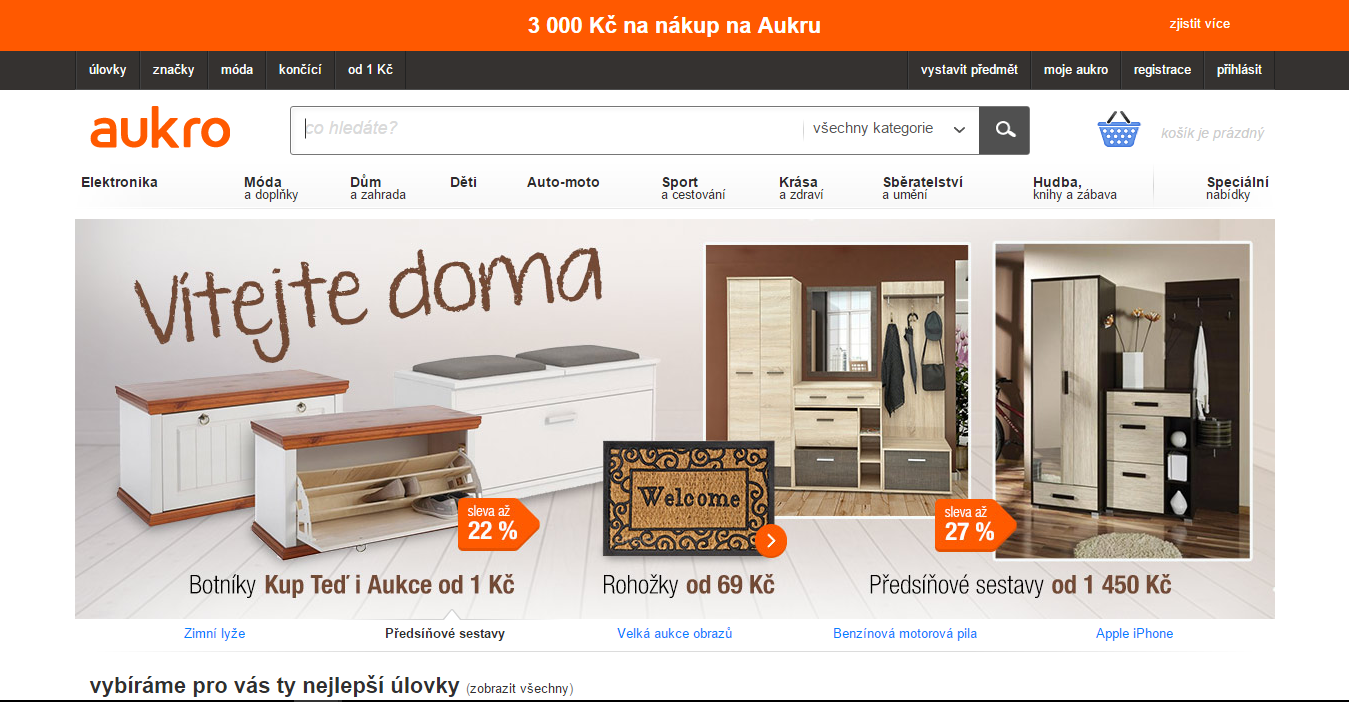
\includegraphics[width=1.0\textwidth]{media/aukro/home.png}
    \caption{Hlavní stránka webu aukro.cz}
    \label{fig:aukro:home}
\end{figure}
\subsubsection*{Pozitiva}
\begin{itemize}
    \item[+] \textbf{Co hledáte?} -- Nejdůležitější prvek (vyhledávání) úvodní stránky je dostatečně velký a je na místě, kde ho uživatelé očekávájí.
    \item[-] \textbf{Kategorie} -- Dobré řešení a při najetí myší se kromě podkategorií zobrazí i populární kategorie a jedna speciální nabídka zboží. Myslím si, že toto chování způsobí, že si nějaká podskupina uživatelů nakoupí i něco, co předtím nechtěli, nebo to nebylo jejich prioritou.
\end{itemize}
\subsubsection*{Negativa}
\begin{itemize}
    \item[-] \textbf{Poutač} -- Velký poutač na speciální akce aukra. Pokud chce uživatel vidět nějaké zboží, které mu vybralo aukro, nebo naposledy shlédnuté zboží, tak musí přejít kolečkem myši dlouhý kus stránky.
\end{itemize}


%%%%%%%%%%%%%%%%%%%%%%%%%%%%%%%%%%%%%%%%%%%%%%%%%%%%%%%%%%%%%%%%%%%%%%%%%%%%%%%%%%%%%%%%%%%%%%%%%%%%%%%%%%%%%%%%%%%%%%%%

\newpage
\subsection{Vyhledávání zboží}
\begin{figure}[h]
    \centering
    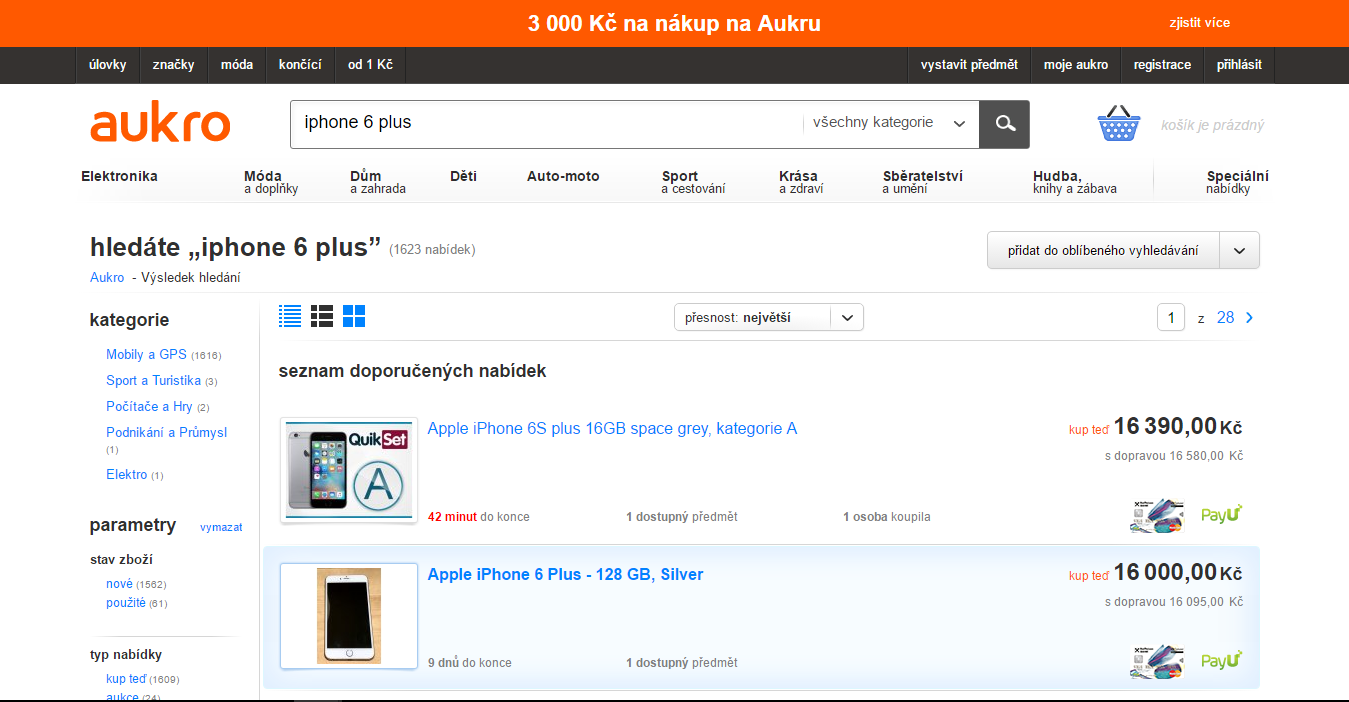
\includegraphics[width=1.0\textwidth]{media/aukro/search.png}
    \caption{Vyhledávání zboží na webu aukro.cz}
    \label{fig:aukro:search}
\end{figure}
\subsubsection*{Pozitiva}
\begin{itemize}
    \item[+] \textbf{Cena i s dopravou} -- Na stránce je přímo zobrazená i cena s dopravou. Uživatel cítí určitou transparentnost a nemusí si tyto informace vyhledávat sám.
\end{itemize}
\subsubsection*{Negativa}
\begin{itemize}
    \item[-] \textbf{Málo informací o zboží} -- O konkrétním zboží se člověk kromě názvu moc nedozví. Místo na alespoň pár detailů tam přitom existuje.
    \item[-] \textbf{Málo nabídek} -- Dvě nabídky zaberou celou stránku ve výchozím nastavení.
    \item[-] \textbf{Chaotické rozhraní} -- Rozhraní je chaotické a neuspořádané.
\end{itemize}


%%%%%%%%%%%%%%%%%%%%%%%%%%%%%%%%%%%%%%%%%%%%%%%%%%%%%%%%%%%%%%%%%%%%%%%%%%%%%%%%%%%%%%%%%%%%%%%%%%%%%%%%%%%%%%%%%%%%%%%%

\newpage
\subsection{Detail zboží}
\begin{figure}[h]
    \centering
    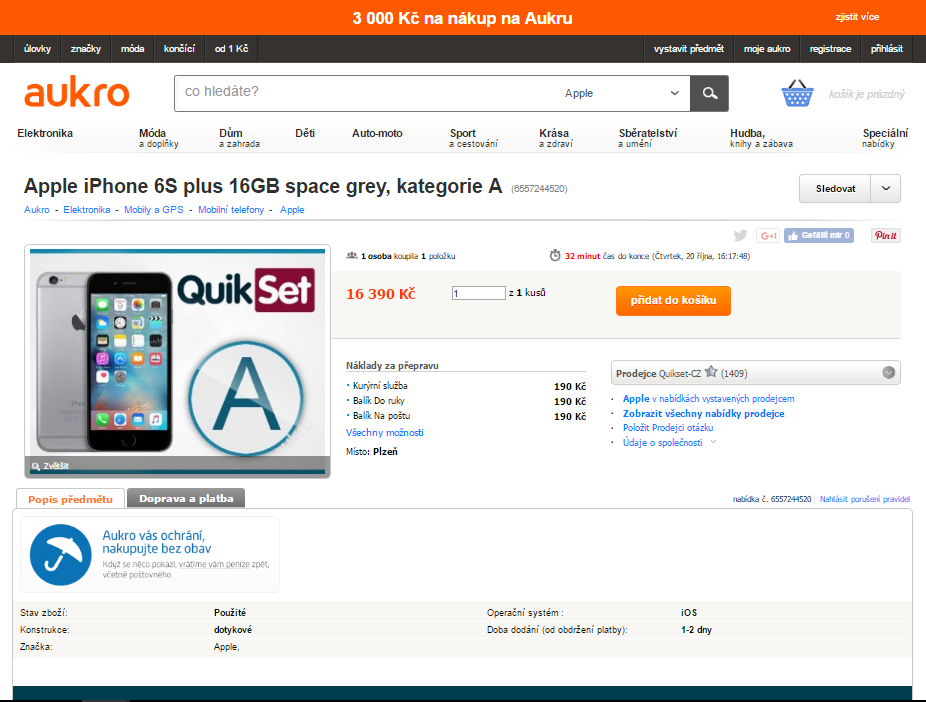
\includegraphics[width=1.0\textwidth]{media/aukro/detail.png}
    \caption{Detail zboží na webu aukro.cz}
    \label{fig:aukro:detail}
\end{figure}
\subsubsection*{Pozitiva}
\begin{itemize}
    \item[+] \textbf{Nevidím}
\end{itemize}
\subsubsection*{Negativa}
\begin{itemize}
    \item[-] \textbf{Neobsahuje moc detailů} -- Detaily sa nacházejí až po delším kuse stránky.
    \item[-] \textbf{Hodnocení prodejců} -- Sice se hodnocení prodejců na stránce nachází, ale výrazně je viditelnější až po rozkliknutí.
    \item[-] \textbf{Chaotické rozhraní} -- Problém uživatelského rozhraní zůstává.
\end{itemize}


%%%%%%%%%%%%%%%%%%%%%%%%%%%%%%%%%%%%%%%%%%%%%%%%%%%%%%%%%%%%%%%%%%%%%%%%%%%%%%%%%%%%%%%%%%%%%%%%%%%%%%%%%%%%%%%%%%%%%%%%

\newpage
\subsection{Profil prodejce}
\begin{figure}[h]
    \centering
    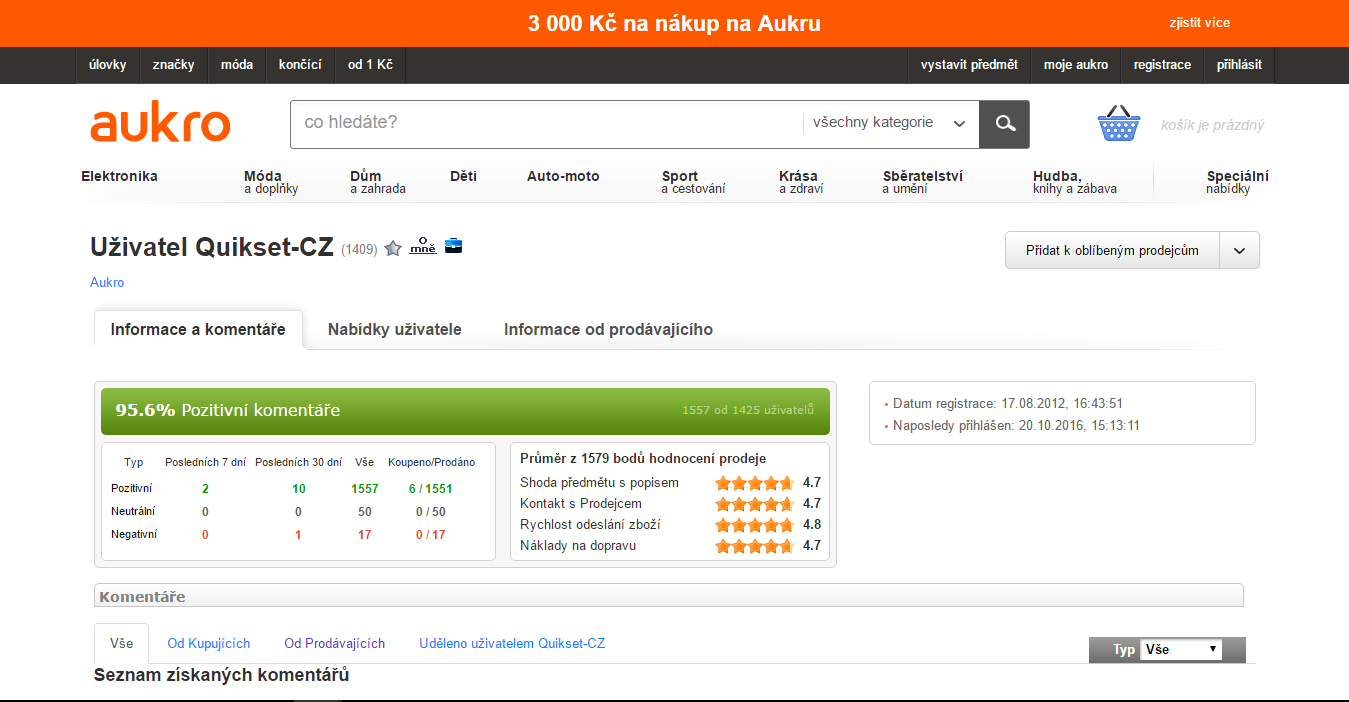
\includegraphics[width=1.0\textwidth]{media/aukro/profile.png}
    \caption{Profil prodejce na webu aukro.cz}
    \label{fig:aukro:profile}
\end{figure}
\begin{figure}[h]
    \centering
    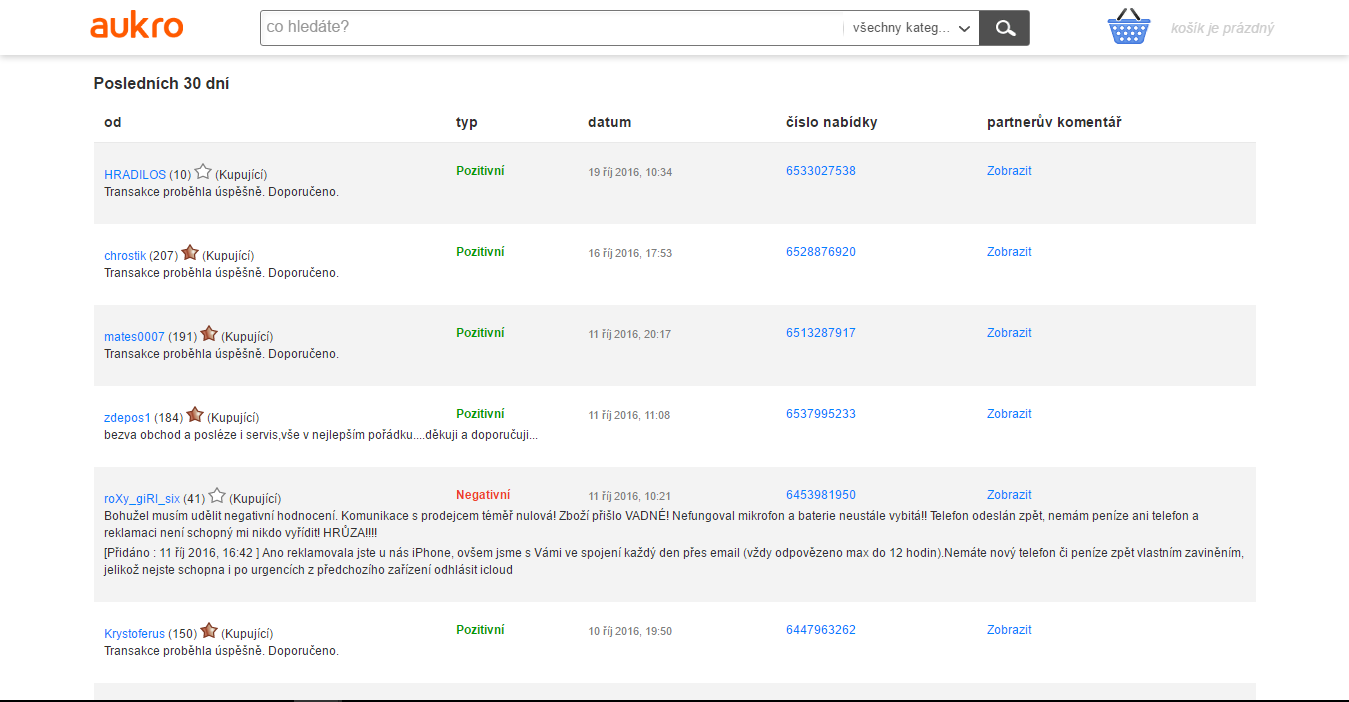
\includegraphics[width=1.0\textwidth]{media/aukro/profile2.png}
    \caption{Recenze uživatele na webu aukro.cz}
    \label{fig:aukro:profile2}
\end{figure}
\subsubsection*{Pozitiva}
\begin{itemize}
    \item[+] \textbf{Historie hodnocení/komentářů} -- Možnost přečíst si kdo byl jak spokojený s daným prodejcem.
\end{itemize}
\subsubsection*{Negativa}
\begin{itemize}
    \item[-] \textbf{Nepřehlednost} -- Problémy s rozhraním se projevují i na této stránce. Nedá se vytvořit si závěry bez dlouhého kroucení kolečkem myši.
\end{itemize}


%%%%%%%%%%%%%%%%%%%%%%%%%%%%%%%%%%%%%%%%%%%%%%%%%%%%%%%%%%%%%%%%%%%%%%%%%%%%%%%%%%%%%%%%%%%%%%%%%%%%%%%%%%%%%%%%%%%%%%%%

\newpage
\subsection{Shrnutí}
Úpřímě řečeno jsem při rešeršování aukro.cz nabudil pocit, že chci z dané webové aplikace co nejdříve odejít. Z mých očekávání se nesplnilo nic a tak se musím poučit z chyb, kterých se dopustili. Konkrétně je to:
\begin{itemize}
    \item \textbf{Chaotické rozhraní}
    \item \textbf{Nedetailnost}
    \item \textbf{Málo poskytnutých informací}
\end{itemize}

Z mého pohledu se jeví být zajímavou funkcí \textbf{historie komentářů}, kdy si uživatel může vytvořit názor o prodejci . Chci však, aby mé rozhraní bylo přehledné a určitě aby poskytovalo všechny potřebné detaily. To pro mě znamená: jaká je daná nabídka, jak daleko je vzdálená a jaké hodnocení má prodejce - a to vše na jednom místě.